\chapter{Fundamentação Teórica}
\label{cap_fundamentacao-teorica}

Este capítulo aborda os conceitos e teorias fundamentais que embasam este estudo. A compreensão desses conceitos é essencial para entender as técnicas e metodologias adotadas ao longo deste trabalho. Inicialmente, é discutida a evolução da Inteligência Artificial (IA). Em seguida, é focado no subcampo da IA denominado \textit{AIOps} (Inteligência Artificial para Operações de TI), que integra IA e análise de dados visando aprimorar as operações de TI. A familiaridade com IA e AIOps é vital para perceber como essas tecnologias podem ser aplicadas em ambientes de TI, potencializando a detecção de anomalias e a análise preditiva de séries temporais.

\section{Revisão Sistemática da Literatura}
\label{cap_revisao-sistematica}

A Revisão Sistemática da Literatura é uma abordagem metodológica que busca identificar, avaliar e interpretar todas as pesquisas relevantes sobre um tema específico. Distingue-se por sua metodologia rigorosa e bem definida, que pode ser replicada e auditada, conferindo maior confiabilidade ao processo utilizado \cite{tranfield2003systematic}.

Essa metodologia é empregada para coletar e sintetizar evidências empíricas que atendam a critérios de inclusão pré-estabelecidos \cite{kitchenham2007guidelines}. O processo envolve a definição de questões de pesquisa pertinentes, a seleção e avaliação qualitativa dos estudos, a extração de dados, a síntese e apresentação da documentação dos achados.

\subsection{Técnicas para Revisão Sistemática da Literatura}
\label{subcap_tec_rev-sistematica}

A Revisão Sistemática é fundamental na pesquisa acadêmica, pois oferece uma visão holística do conhecimento existente, destacando lacunas que podem ser objeto de futuras investigações \cite{petticrew2006systematic}. Além disso, evita a duplicação de esforços, evidenciando pesquisas prévias sobre o tema.

A elaboração de uma revisão sistemática é iniciada com a definição de um protocolo rígido de pesquisa. Neste protocolo, são estabelecidos critérios de inclusão e exclusão, as bases de dados a serem consultadas e as estratégias de busca a serem adotadas \cite{biolchini2005systematic}. A figura \ref{fig:processo_rev_sistematica} apresenta uma ilustração mais detalhes sobre procedimento adotado neste estudo:

\begin{figure}[H]
    \centering
    \caption{Procedimento adotado para realização da Revisão Sistemática da Literatura.}
    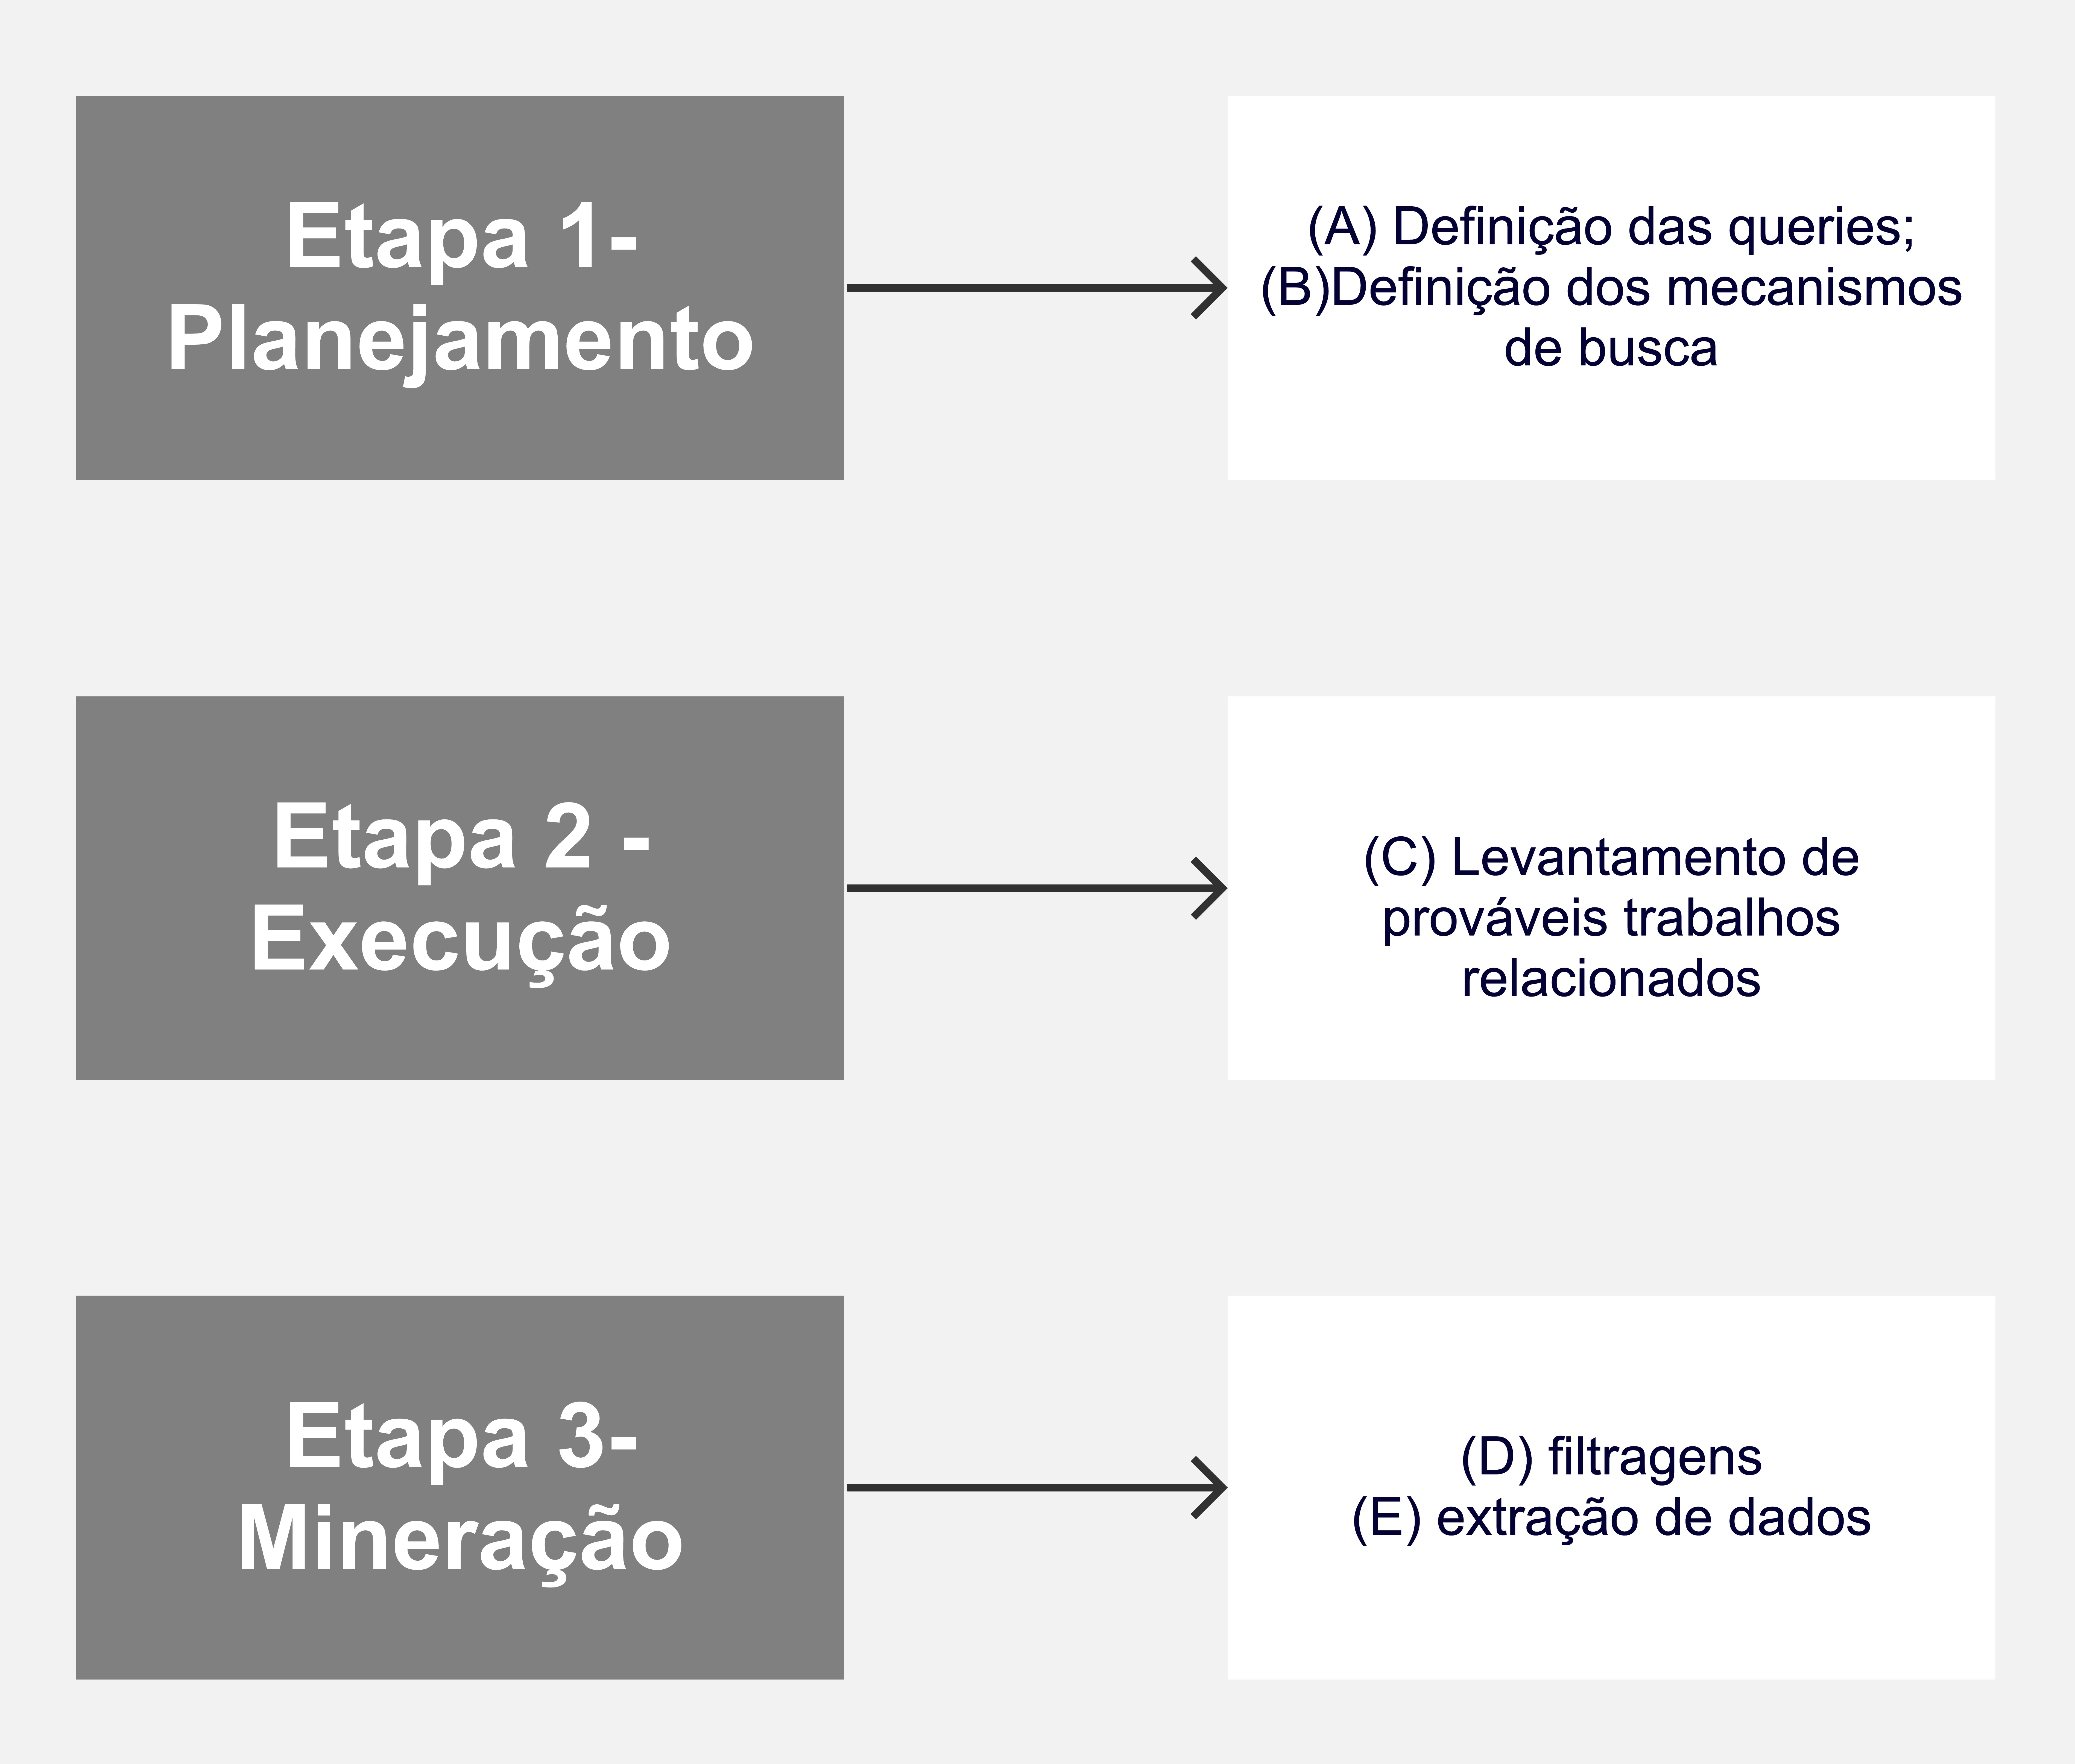
\includegraphics[width=10cm,height=\textwidth,keepaspectratio]{Dissertation//Weslley-Rosalem_Dissertacao-Estudos-Especiais-Quali//2-images/2- Fluxograma mestrado.jpg}
    \newline
    \centering{Fonte: Elaborado pelo autor}
    \label{fig:processo_rev_sistematica}
\end{figure}

As etapas apresentadas na figura \ref{fig:processo_rev_sistematica} são detalhadas a seguir:

\begin{enumerate}
    
    \item As \textit{queries}\footnote{\textit{Queries} são instruções ou expressões usadas para recuperar informações de um banco de dados. Elas são frequentemente escritas em uma linguagem de consulta de banco de dados como SQL.} são \textit{strings}\footnote{\textit{Strings} são sequências de caracteres usadas para representar texto em programação e computação. Elas são fundamentais para o processamento de texto, pesquisa e muitas outras aplicações.}
 que estabelecem critérios para a seleção de artigos. Nesta pesquisa, o foco foi em artigos cujo título ou \textit{keywords}\footnote{\textit{Keywords} são palavras ou frases que resumem o conteúdo principal de um texto, documento ou base de dados. Elas são frequentemente usadas em buscas para encontrar informações relevantes.}
 incluíssem a palavra \textit{AIOPs}. Além disso, restringiu-se o período de publicação entre 2018 e o primeiro semestre de 2023.
    
    \item Dada a reconhecida relevância em Ciência da Computação, especialmente em Redes de Computadores, monitoramento e observabilidade, duas bases de pesquisa científica foram selecionadas: IEEExplore\footnote{https://ieeexplore.ieee.org/} e ACM \textit{Digital Library}\footnote{https://dl.acm.org/}.
    
    \item A execução das \textit{queries} nas bases mencionadas resultou em 80 artigos. A distribuição dos artigos por ano de publicação é ilustrada na Figura \ref{fig:grafico_num_papers}:
      \begin{figure}[H]
    \centering
    \caption{Distribuição dos artigos por ano de publicação.} 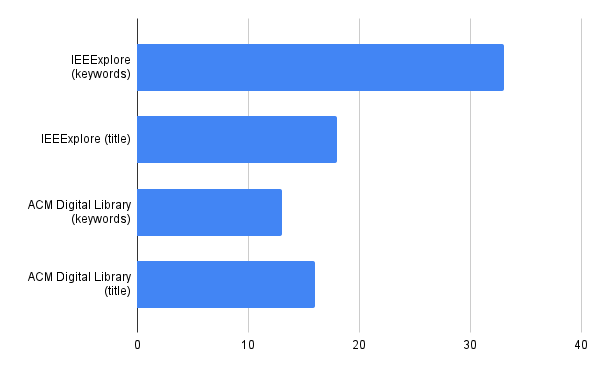
\includegraphics[width=13cm,height=\textwidth,keepaspectratio]{2-images/artigos-bars-horizontal.png}
    \newline \centering{ Fonte: Elaborado pelo autor}\label{fig:grafico_num_papers}
    \end{figure}
    
   \item Durante a filtragem, foram removidos artigos duplicados ou inacessíveis, totalizando 22 duplicados e 2 inacessíveis. Dos 56 artigos remanescentes, 35 não se alinhavam diretamente ao escopo desta dissertação. Portanto, após a filtragem, 21 artigos foram reconhecidos como estreitamente relacionados ao tema proposto. A Figura \ref{fig:grafico_processamento_papers} ilustra este processo:

    \begin{figure}[H]
    \centering
    \caption{Detalhamento do resultado após os processos de filtragem dos artigos.} 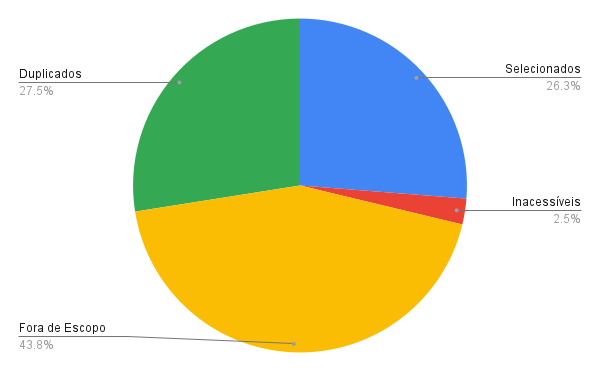
\includegraphics[width=11cm,height=\textwidth,keepaspectratio]{2-images/chart-2.png}
    \newline \centering{ Fonte: Elaborado pelo autor}\label{fig:grafico_processamento_papers}
    \end{figure}    

\item A última etapa envolveu a extração das informações mais relevantes dos artigos selecionados. Para identificar tendências, as seguintes informações foram extraídas:
     \begin{itemize}
         \item Tipo de modelo: técnicas de \textit{machine learning} empregadas ou propostas;
         \item \textit{Dataset}\footnote{Um \textit{dataset} é uma coleção de dados, geralmente apresentada em formato tabular, que serve como entrada para algoritmos de aprendizado de máquina e análise estatística.} : bases de dados utilizadas nos testes;
         \item Arquitetura: arquiteturas propostas;
         \item \textit{Feature selection}\footnote{\textit{Feature Selection} é o processo de selecionar um subconjunto de características relevantes para uso em modelagem. A seleção de características eficaz pode melhorar o desempenho do modelo e reduzir a complexidade computacional.} :
         \item  \textit{features}\footnote{\textit{Features} são variáveis individuais que atuam como entradas em modelos de aprendizado de máquina. Cada feature representa uma dimensão específica de dados que o algoritmo pode usar para aprender.} selecionadas;
         \item Resultados: conclusões alcançadas pelos autores, como RMSE e MAE; e
         \item Metodologia: recursos utilizados na criação do modelo de identificação de anomalias e predição, incluindo linguagens e \textit{softwares}.
     \end{itemize}

\end{enumerate}

Os artigos selecionados foram sintetizados, destacando-se os elementos mais pertinentes ao contexto desta pesquisa. A organização dos estudos foi feita conforme:

\begin{itemize}
    \item Não foram encontrados trabalhos correlatos no ano de 2018. Esta afirmação indica que, após uma busca sistemática na literatura utilizando palavras-chave e critérios específicos, não foram identificados estudos ou publicações relacionadas ao tema da dissertação no ano de 2018;
    \item Trabalhos correlatos de 2019 na Subseção \ref{trab_correlatos_19};
    \item Trabalhos correlatos de 2020 na Subseção \ref{trab_correlatos_20};
    \item Trabalhos correlatos de 2021 na Subseção \ref{trab_correlatos_21};
    \item Trabalhos correlatos de 2022 na Subseção \ref{trab_correlatos_22};
    \item Trabalhos correlatos de 2023 na Subseção \ref{trab_correlatos_23};
\end{itemize}

A Figura \ref{fig:diagrama_detalhado_rev_sistematica} ilustra o processo completo da Revisão Sistemática da Literatura, desde a definição das \textit{queries} até a extração das informações cruciais:


\begin{figure}[H]
\centering
\caption{Procedimento adotado para realização da Revisão Sistemática da Literatura.} 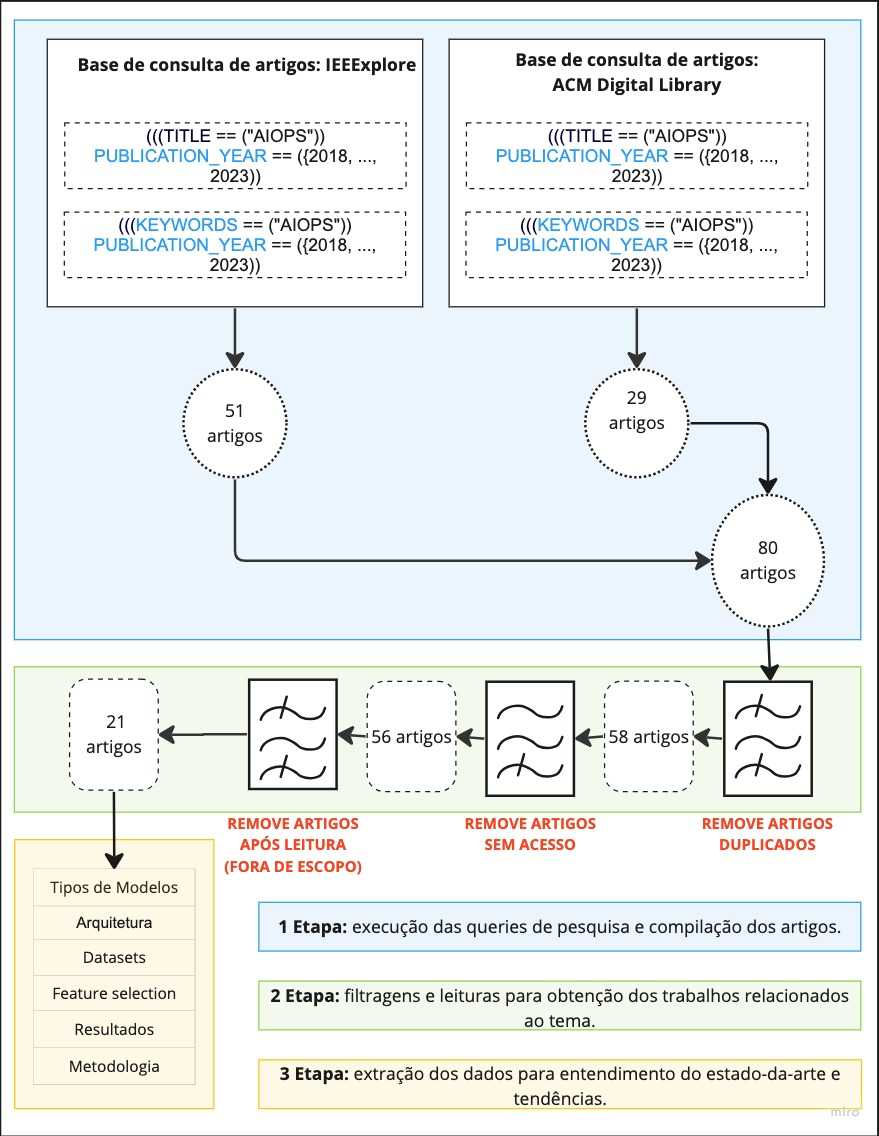
\includegraphics[width=9cm,height=\textwidth,keepaspectratio]{2-images/Fluxograma-papers.png}
\newline \centering{Fonte: Elaborado pelo autor}\label{fig:diagrama_detalhado_rev_sistematica}
\end{figure}    
    

\subsection{Trabalhos Correlatos - ano de 2019}\label{trab_correlatos_19}

No artigo de \cite{8752866}, os autores exploram a aplicação de Inteligência Artificial nas Operações de TI (AIOps) para detectar anomalias com base em registros de \textit{distributed tracing}. Estes registros fornecem informações detalhadas sobre a disponibilidade e o tempo de resposta dos serviços. A abordagem proposta foca na detecção de anomalias no tempo de resposta usando aprendizado não supervisionado. Eles empregam técnicas de modelagem de dados de aprendizado profundo e avaliam a precisão e o desempenho da abordagem em ambientes de teste e produção. A combinação de GRUs (Unidades Recorrentes de Memória) e \textit{autoencoders} variacionais é destacada como uma técnica promissora para modelar séries temporais complexas.

\subsection{Trabalhos Correlatos - ano de 2020}\label{trab_correlatos_20}

O estudo de \cite{9156101} aborda o desafio de monitorar ambientes de TI complexos, que englobam nuvens privadas e públicas, ambientes de IoT, aplicativos e contêineres. Eles destacam a necessidade de um modelo de contexto em AIOps para gerenciar grandes volumes de dados armazenados em diferentes formatos. O \textit{framework} proposto é estruturado em cinco camadas: aquisição, gerenciamento, análise, apresentação de dados e respostas automatizadas. O \textit{Monitoring Resource Model} (MRM) é um componente central desse \textit{framework}. Para a análise de dados, é proposto um modelo de aprendizado de máquina baseado em redes neurais, especificamente o \textit{Long-Short-Term-Memory} (LSTM).

\cite{9311349} discute a importância do aprendizado de máquina, especialmente no contexto de AIOps, para descobrir relacionamentos entre objetos e processos em infraestruturas de TI convergentes. O estudo enfatiza a necessidade de técnicas de aprendizado de máquina para identificar padrões e sequências em grandes volumes de eventos. A arquitetura proposta foca na análise e aprendizado de máquina para processar dados de diversos dispositivos e instrumentos de TI.

O objetivo do estudo apresentado por \cite{9443765} é propor uma rede neural dinâmica para prever fluxos de dados de séries temporais em cenários de AIOps. Os modelos de aprendizado de máquina discutidos incluem \textit{MWNN (Multi-Way Neural Network), WNN (Wavelet Neural Network)} e LSTM. Os dados utilizados durante os testes incluem conjuntos de dados de CPUs com diferentes capacidades. Os resultados mostram uma comparação do consumo de recursos para MWNN, WNN e LSTM quando alcançam o mesmo desempenho.



\subsection{Trabalhos Correlatos - ano de 2021}\label{trab_correlatos_21}

No estudo conduzido por \cite{9516546}, os autores propõem uma abordagem inovadora que combina múltiplos métodos integrados para prever a capacidade de recursos. Utilizando o modelo de aprendizado de máquina LSTM (\textit{Long Short-Term Memory}), o estudo demonstra como, com base nos dados históricos, é possível fornecer previsões precisas sobre o uso de recursos de TI, como CPU, disco rígido e memória. Esta abordagem tem potencial para otimizar a gestão de recursos, garantindo que os sistemas permaneçam estáveis e confiáveis.

\cite{9605403} introduz o conceito de \textit{Machine Reasoning} (MR) e destaca seu papel vital na melhoria das Operações de Inteligência Artificial (AIOps) para Redes Baseadas em Intenções. MR é uma subárea da Inteligência Artificial (IA) que se concentra em capturar e utilizar o conhecimento humano através de linguagens semânticas. Esta abordagem complementa a Aprendizagem de Máquina (ML) ao fornecer inferências precisas baseadas no conhecimento adquirido. O estudo apresenta cenários em que MR em AIOps pode ser utilizado para automatizar e aprimorar a identificação da causa raiz de problemas em redes de computadores.

O artigo de \cite{9678534} apresenta o método AID (\textit{Aggregated Intensity of Dependency}) como uma solução eficiente para prever a intensidade das dependências em sistemas de nuvem em larga escala. Os autores utilizam dados simulados e industriais para testar a eficácia do método proposto. Os resultados mostram que o AID é capaz de medir com precisão a intensidade das dependências, superando outras abordagens comparativas.

\cite{9680514} discute o \textit{design} e a implementação de recursos para migrar dados de sistemas de monitoramento antigos para instâncias do \textit{Prometheus} usando o \textit{framework Ananke}. Além disso, o estudo propõe uma estratégia de dimensionamento automático baseada na previsão de picos de tráfego usando o modelo \textit{Facebook} \textit{Prophet}. A abordagem é voltada para monitorar e modelar aplicações nativas de nuvem, com foco em métricas de desempenho em tempo real e estratégias de otimização.

\subsection{Trabalhos Correlatos - ano de 2022}\label{trab_correlatos_22}

\cite{9492267} introduz o TSAGen, uma ferramenta inovadora de geração de séries temporais. Esta ferramenta permite aos pesquisadores gerar dados sintéticos, fornecendo uma fonte de dados confiável para avaliar o desempenho de algoritmos de detecção de anomalias. O TSAGen foi projetado para enfrentar desafios como a geração de diversas anomalias, ajuste da gravidade das anomalias e controle das características dos KPIs gerados.

No estudo de \cite{9746242}, os autores propõem uma rede neural profunda, a CDX-Net, para previsão de séries temporais multivariadas no contexto de AIOps. A arquitetura proposta do CDX-Net incorpora módulos avançados, como ASPP, SRM, CAM, GRU, transformador e AB, para aprimorar os procedimentos de extração e fusão de características.

\cite{9746416} apresenta uma solução para o Desafio ICASSP-SPGC-2022 AIOps, focando na inferência precisa de combinações em \textit{root cause analysis} (RCA). O documento detalha os desafios encontrados nos dados da competição e propõe uma estrutura robusta para resolver o problema, incluindo a introdução de \textit{TextCNN}.

O estudo de \cite{9789784} propõe uma abordagem para gerar relatórios de falhas legíveis por humanos em sistemas de TIC. A abordagem utiliza o modelo LSTM para séries temporais multivariadas e gera um relatório de falha em formato de texto. Os autores testam a eficácia e o desempenho do método proposto usando dados coletados de um sistema de microsserviços em um \textit{cluster Kubernetes} (k8s).


\cite{9825776} apresenta uma discussão profunda sobre a representação gráfica para o DevOps em aplicações baseadas em aprendizado de máquina, também conhecida como MLOps. Os autores exploram meticulosamente as fases do MLOps, desde o planejamento, onde são identificados o problema a ser resolvido e os dados disponíveis, até a seleção de abordagens de análise de dados e algoritmos adequados. A fase de codificação é destacada, onde o sistema e o código de ML são implementados e validados. A fase de validação é discutida em detalhes, enfatizando a avaliação do desempenho do modelo de ML com novos dados. O artigo também destaca a necessidade imperativa de um processo de MLOps integrado e delinea os desafios associados à adoção prática do MLOps.

\cite{9835411} propõe um framework de dimensionamento automático proativo inovador chamado \textit{RobustScaler}, especialmente projetado para cenários de computação em nuvem. O estudo é direcionado para o desenvolvimento de um \textit{framework} que não apenas gera decisões de mudança e elasticidade, mas também otimiza o equilíbrio entre custo e Qualidade de Serviço (QoS). O modelo proposto é robusto, capaz de lidar com ruídos, dados ausentes e anomalias. O algoritmo de Método dos Multiplicadores de Direção Alternada (ADMM) é usado para treinar o modelo, que captura tanto a periodicidade quanto a estocasticidade das chegadas de consultas. A arquitetura do \textit{framework} é composta por componentes essenciais, como detecção de periodicidade, modelagem histórica de chegadas de consultas, previsão de chegada de consultas e plano de dimensionamento.

\cite{9892264} introduz um \textit{framework} inovador baseado em aprendizado federado, o EFL-WP, projetado especificamente para previsão de carga de trabalho em ambientes inter-nuvem. O \textit{framework} visa colaborar na formação de modelos de \textit{machine learning} para previsão de carga de trabalho, garantindo que informações sensíveis não sejam compartilhadas. Os autores sugerem o uso de modelos LSTM para prever métricas de desempenho, como utilização da CPU e memória. A arquitetura proposta é composta por um coordenador que agenda tarefas de treinamento e orquestra os treinadores, enquanto os treinadores usam seus dados para treinar modelos locais.

\cite{9978983} apresenta o método "\textit{PUTraceAD}" \textit{Positive-Unlabeled}, uma abordagem inovadora para detecção de anomalias em \textit{tracing} de microsserviços. A arquitetura proposta é tripartida, envolvendo \textit{Embedding} de \textit{Span}, Construção de Grafo de Rastros e Treinamento do Modelo. Utilizando uma GNN (\textit{Graph Neural Network}) e aprendizado PU, o método é capaz de detectar anomalias em \textit{tracing} com precisão. O conjunto de dados usado, \textit{TrainTicket}, é um sistema de referência de microsserviços, e os experimentos foram conduzidos em um \textit{cluster Kubernetes}. Os resultados dos experimentos avaliam a eficácia e eficiência do \textit{PUTraceAD}, bem como o impacto de diferentes configurações.

\cite{9985105} discute o Sistema de Gerenciamento de Dependências, ou \textit{Dependency Management System} (DMS), uma solução abrangente para gerenciar dependências de serviços em sistemas em nuvem. O DMS é uma plataforma \textit{end-to-end} que suporta todo o ciclo de vida para garantir a confiabilidade do serviço, desde a implantação inicial até a otimização arquitetural proativa e a mitigação reativa de falhas. Os dados usados nos testes do DMS abrangem uma variedade de fontes, incluindo informações de dependência coletadas de \textit{trancing} distribuído, arquivos de configuração, consultas do orquestrador de serviços e relatórios de dependência de implantação.

\cite{10004053} aborda questões relacionadas à implementação da observabilidade em sistemas de informações hospitalares (HIS). O artigo apresenta uma pesquisa literária detalhada e fornece um resumo abrangente de conceitos relacionados, incluindo definições de monitoramento e HIS, requisitos e soluções em cenários específicos. A arquitetura proposta integra microsserviços e AIOps, com indicadores-chave (KPIs) como qualidade e escala de dados. O documento também oferece sugestões valiosas para os departamentos de TI dos hospitais sobre como abordar essas questões.

\cite{10020986} realiza uma análise detalhada de AIOps na gestão unificada de resiliência de dados em data lakehouses. O artigo propõe soluções inovadoras para prever violações do Recovery Point Objective (RPO) e fornecer sugestões valiosas aos SREs sobre como configurar recursos do sistema para evitar tais violações. Utilizando aprendizado supervisionado em conjunto com análise de séries temporais, o artigo propõe um modelo de aprendizado de máquina que combina métodos de aprendizado online e offline e filtragem de solicitações previstas para garantir a estabilidade das solicitações futuras.



\subsection{Trabalhos Correlatos - ano de 2023}\label{trab_correlatos_23}

%56
Em \cite{10098585}, os autores apresentam uma análise detalhada sobre a implementação de \textit{baselines} utilizando a linguagem de programação \textit{Python}. Eles escolhem a regressão linear como o modelo de aprendizado de máquina para sua análise. O artigo aborda profundamente as questões de pesquisa, o design experimental meticuloso, a aplicação na análise de desempenho e as distribuições de latência. Os autores também discutem o uso de cargas de trabalho que variam continuamente e fornecem \textit{insights} sobre a configuração experimental, destacando a importância de uma abordagem sistemática para garantir resultados precisos e confiáveis.

%57
\cite{10113794} oferece uma visão abrangente do desenvolvimento do sistema de detecção de \textit{outlier} denominado \textit{OutSpot}. Este sistema é especialmente projetado para \textit{datacenters} de alto desempenho e alta criticidade, que são primordialmente responsáveis pelo fornecimento de \textit{streaming} de vídeos. O principal objetivo do sistema é detectar \textit{outliers} nos KPIs coletados desses \textit{datacenters}. O modelo de ML adotado é uma combinação inovadora de \textit{Hierarchical Agglomerative Clustering} (HAC) com Conditional Variational Autoencoder (CVAE). O HAC é utilizado para agrupar os KPIs com base em seus padrões distintos. Posteriormente, as informações de agrupamento de cada KPI são incorporadas ao método. Esta abordagem integrada permite que o \textit{OutSpot} detecte \textit{outliers} para KPIs em larga escala, mesmo quando esses KPIs apresentam padrões variados. A arquitetura proposta para o \textit{OutSpot} é meticulosa, dividindo os conjuntos de dados coletados em conjuntos de treinamento e teste. O conjunto de treinamento é composto por dados coletados ao longo dos primeiros 7 dias, enquanto o conjunto de teste contém dados do último dia. Este último conjunto é rotulado cuidadosamente por operadores experientes utilizando uma ferramenta desenvolvida pelos próprios autores. O processo de rotulação dos \textit{outliers} é rigoroso, envolvendo três operadores, e a decisão final é tomada apenas quando os rótulos fornecidos por eles divergem.



% Please add the following required packages to your document preamble:
% \usepackage{longtable}
% Note: It may be necessary to compile the document several times to get a multi-page table to line up properly
\begin{longtable}{|p{2.5cm}|p{4cm}|p{8cm}|}
\caption{Características da análise sistemática da literatura}
\label{tab:res-anali-sistematica}\\
\hline
\textbf{Ano de Publicação} & \textbf{Autores}         & \textbf{Tópico Principal}                                                                              \\ \hline
\endfirsthead
%
\endhead
%
2019              & \cite{8752866}  & Detecção de anomalias usando \textit{Distributed Tracing} e \textit{Deep Learning} em AIOps                     \\ \hline
2020              & \cite{9156101}  & Monitoramento de ambiente de TI complexo com modelo de contexto                               \\ \hline
2020              & \cite{9311349}  & Redução de incidentes em infraestruturas de TI convergentes através de aprendizado de máquina \\ \hline
2020              & \cite{9443765}  & Previsão de fluxos de dados de séries temporais em cenários de AIOps                          \\ \hline
2021              & \cite{9516546}  & Previsão da capacidade de recursos usando LSTM                                                \\ \hline
2021              & \cite{9605403}  & Melhoria das Operações de IA para Redes Baseadas em Intenções usando \textit{Machine Reasoning}        \\ \hline
2021              & \cite{9678534}  & Previsão da intensidade de dependências em sistemas em nuvem                                  \\ \hline
2021              & \cite{9680514}  & Migração de dados de sistemas de monitoramento antigos para instâncias do \textit{Prometheus}          \\ \hline
2022              & \cite{9492267}  & Geração de séries temporais para avaliação de algoritmos de detecção de anomalias             \\ \hline
2022              & \cite{9746242}  & Previsão de séries temporais multivariadas em AIOps                                           \\ \hline
2022              & \cite{9746416}  & Inferência precisa de combinações em \textit{root} cause \textit{analysis}                                      \\ \hline
2022              & \cite{9789784}  & Geração de relatórios de falhas legíveis por humanos em sistemas de TIC                       \\ \hline
2022              & \cite{9825776}  & Representação gráfica para o \textit{DevOps}\footnote{\textit{DevOps} é uma filosofia e prática de engenharia de software que visa unificar o desenvolvimento de software (\textit{Dev}) e a operação de software (\textit{Ops}). O principal objetivo de DevOps é encurtar o ciclo de vida do desenvolvimento de sistemas, proporcionando entrega contínua de alta qualidade, e, assim, melhorar a colaboração e a comunicação entre as equipes de desenvolvimento e operações. *DevOps* integra métodos ágeis, automação, integração contínua, entrega contínua e monitoramento contínuo do software em operação.}
 em aplicações baseadas em aprendizado de máquina (MLOps)  \\ \hline
2022              & \cite{9835411}  & \textit{Framework} de dimensionamento automático proativo para computação em nuvem                     \\ \hline
2022              & \cite{9892264}  & Previsão de carga de trabalho em ambientes de inter-nuvem usando aprendizado federado         \\ \hline
2022              & \cite{9978983}  & Detecção de anomalias em \textit{tracing} de microsserviços usando GNN e aprendizado PU                \\ \hline
2022              & \cite{9985105}  & Gerenciamento de dependências de serviços em sistemas em nuvem                                \\ \hline
2022              & \cite{10004053} & Implementação da observabilidade em sistemas de informações hospitalares (HIS)                \\ \hline
2022              & \cite{10020986} & Gestão unificada de resiliência de dados em data \textit{lakehouses}                                   \\ \hline
2023              & \cite{10098585} & Implementação de \textit{baselines} usando \textit{Python} e regressão linear                                   \\ \hline
2023              & \cite{10113794} & Detecção de \textit{outlier} para \textit{datacenters} com alto nível de desempenho e alta criticidade          \\ \hline
\end{longtable}


\section{Arquitetura \textit{Transformer}} \label{sec-arquitetura-transformer}

A arquitetura \textit{Transformer} foi pioneiramente introduzida no artigo \textit{"Attention Is All You Need"} por \cite{vaswani2017attention}. Esta arquitetura representou uma mudança paradigmática no processamento de sequências. Ao contrário dos modelos tradicionais, como as redes neurais convolucionais (CNNs) e as redes neurais recorrentes (RNNs), especialmente em tarefas de processamento de linguagem natural (PLN),  eliminando a necessidade de recorrência e convoluções, centrando-se exclusivamente em mecanismos de atenção, que permite ao modelo ponderar diferentes segmentos da entrada com base em sua relevância para a tarefa em questão, e desta maneira para discernir dependências contextuais entre os dados de uma maneira mais eficiente e escalável. 


As redes neurais \textit{feed-forward} formam a base da arquitetura \textit{Transformer}, que em sua essência é composto por dois componentes principais: um codificador (\textit{encoder}) e um decodificador (\textit{decoder}). Cada um desses componentes é uma pilha de camadas idênticas que contêm sub-camadas \textit{feed-forward}. Sua estrutura é explicada nas subseções seguintes.

\subsection{Redes Neurais Feed-forward}
As redes neurais \textit{feed-forward} dentro das sub-camadas do \textit{Transformer} são relativamente simples, consistindo geralmente em duas camadas lineares com uma ativação não-linear entre elas. A função destas redes \textit{feed-forward} é transformar os dados de forma independente em cada posição.

\subsection{Mecanismo de Atenção}
O principal elemento desta arquitetura é o mecanismo de "atenção multi-cabeça". Este mecanismo permite que o modelo pondere diferentes segmentos da sequência de entrada de maneira variável, dependendo da relevância contextual de cada segmento ao gerar cada componente da sequência de saída \cite{vaswani2017attention}. Esse foco adaptativo permite que o modelo capture nuances e dependências sutis em dados sequenciais. Matematicamente, o mecanismo de atenção é formulado como:

\[
\text{Attention}(Q, K, V) = \text{softmax}\left(\frac{QK^T}{\sqrt{d_k}}\right) V
\]

Nesta formulação, \(Q\), \(K\), e \(V\) representam as matrizes de consulta, chave e valor, respectivamente. \(d_k\) denota a dimensionalidade das chaves. Este mecanismo sofisticado permite que o modelo \textit{Transformer} aloque atenção diferenciada a diferentes segmentos da entrada, otimizando sua capacidade de modelar relações complexas nos dados \cite{vaswani2017attention}.

\subsection{Codificador e Decodificador}
O codificador é a primeira etapa da arquitetura \textit{Transformer} e é responsável por processar e transformar a entrada em uma representação contínua e abstrata. Esta representação é então passada para o decodificador, que a utiliza para gerar a saída desejada. Ambos, codificador e decodificador, são compostos por múltiplas camadas que contêm mecanismos de atenção e redes neurais \textit{feed-forward}, permitindo uma modelagem profunda e abrangente dos dados.

Cada camada no codificador contém duas sub-camadas: a primeira é a atenção multi-cabeça e a segunda é uma rede neural \textit{feed-forward} simples. A rede \textit{feed-forward} é aplicada separadamente e de forma idêntica a cada posição, ou seja, é a mesma operação em todos os elementos da sequência, mas é aplicada de forma independente para cada um.

Além das duas sub-camadas presentes no codificador, cada camada do decodificador possui uma terceira sub-camada que realiza atenção multi-cabeça sobre a saída do codificador. Esta atenção inter-camadas ajuda o decodificador a focar em partes relevantes da entrada ao gerar a saída.


\subsection{Codificação Posicional}
Uma característica distintiva do \textit{Transformer} é a sua capacidade de processar sequências sem depender de recorrência. Para compensar a ausência de uma noção inerente de ordem, o modelo utiliza codificações posicionais. Estas codificações são adicionadas aos \textit{embeddings} de entrada, garantindo que o modelo possa considerar a posição relativa de cada elemento na sequência \cite{vaswani2017attention}.

\subsection{Normalização de Camada}
Para garantir a estabilidade e a eficiência do treinamento, cada sub-camada dentro dos codificadores e decodificadores é acompanhada por uma normalização de camada. Este processo ajusta e estabiliza as ativações, permitindo uma convergência mais rápida e um treinamento mais estável \cite{ba2016layer}. Uma representação simplificada dessa formulação, pode ser dada por:
\[
\text{LayerNorm}(x + \text{Sublayer}(x))
\]

Nesta equação, \(\text{\textit{Sublayer}}(x)\) representa a saída de uma das sub-camadas, como a atenção multi-cabeça ou a rede neural \textit{feed-forward}.


\subsection{Pseudo-código}
Para uma compreensão detalhada e mais profunda da implementação do \textit{Transformer}, um pseudo-código detalhado é fornecido no apêndice \ref{appendix:a}.

\subsection{Desafios e Limitações}
Apesar de suas inúmeras vantagens, o \textit{Transformer} apresenta desafios. Sua complexidade computacional, especialmente em modelos de grande escala, pode ser proibitiva em certos cenários. Além disso, embora o mecanismo de atenção ofereça algum grau de visibilidade sobre o funcionamento do modelo, ele não garante uma interpretabilidade completa, o que pode ser um obstáculo em aplicações que exigem transparência total \cite{jiang2019attention}.


\section{Análise Preditiva com \textit{Transformer}} \label{cap-anal-pre-trans-ts}

A análise preditiva de séries temporais é uma área de pesquisa em rápido crescimento, com aplicações em diversos domínios, desde o setor financeiro até operações de TI. Este estudo adota a arquitetura \textit{Transformer}, que, embora originalmente projetada para tarefas de processamento de linguagem natural \cite{vaswani2017attention}, demonstrou uma capacidade notável de modelar dependências temporais em séries temporais \cite{lim2019temporal}.


\subsection{Arquitetura \textit{Transformer} em Séries Temporais}
O \textit{Time Series Transformer} (TST), é uma extensão especializada do \textit{Transformer}, adaptado para lidar com as nuances e características específicas das séries temporais \cite{lim2019temporal}. Mantendo o mecanismo de atenção, o TST é capaz de capturar dependências temporais em múltiplas escalas, tornando-o ideal para modelar e analisar sequências temporais.

A eficácia do TST é fortemente influenciada pela seleção apropriada de hiperparâmetros. A escolha do número de camadas, dimensão do modelo e número de cabeças de atenção é crucial. Estes parâmetros devem ser meticulosamente ajustados conforme a natureza dos dados e o problema específico para garantir o desempenho ótimo do modelo.

Quando aplicado a métricas de séries temporais, como as armazenadas em sistemas como o \textit{Prometheus}, o TST tem o potencial de discernir padrões intrincados e dependências temporais, facilitando a identificação de anomalias, sazonalidades e a previsão de tendências futuras.  

\subsection{Inteligência Artificial}
A Inteligência Artificial (IA) é uma disciplina interdisciplinar que aspira a criar máquinas capazes de emular comportamentos inteligentes humanos \cite{russell2016artificial}. A IA engloba habilidades como aprendizado a partir de experiências, compreensão de linguagem natural, reconhecimento de padrões e tomada de decisões autônomas. Ela é o resultado da convergência de campos como ciência da computação, matemática, psicologia, neurociência e linguística.

Nos últimos anos, a IA tem experimentado avanços significativos, impulsionados por melhorias em algoritmos, capacidades computacionais avançadas e a disponibilidade de grandes volumes de dados \cite{poole2017artificial}.

O aprendizado de máquina, uma subárea proeminente da IA, foca em desenvolver algoritmos que aprimorem seu desempenho com base nos dados fornecidos \cite{mitchell1997machine}. O aprendizado profundo, uma subdivisão do aprendizado de máquina, tem se destacado em tarefas complexas, como reconhecimento de imagens e processamento de linguagem natural, devido à sua capacidade de modelar relações intrincadas em grandes conjuntos de dados \cite{lecun2015deep}.

\subsection{AIOps}
AIOps, uma abreviação para Inteligência Artificial para Operações de TI, é um conceito introduzido pelo \textit{Gartner}, que se refere à integração de técnicas de IA nas operações de TI \cite{gardner2017artificial}. AIOps visa aprimorar e automatizar aspectos das operações de TI, como monitoramento, gerenciamento e análise de dados, através da combinação de \textit{big data} e aprendizado de máquina.

Com AIOps, as operações de TI podem transitar de uma abordagem reativa para uma proativa. Isso significa que, em vez de apenas responder a problemas após sua ocorrência, é possível antecipar e prevenir problemas, otimizando a eficiência e confiabilidade das operações de TI \cite{sill2019aiops}.

\subsection{Séries Temporais e Prometheus}
Séries temporais são conjuntos ordenados de dados coletados em intervalos sequenciais e regulares \cite{shumway2017time}. No contexto de TI, elas são essenciais para monitorar e otimizar sistemas, com métricas como uso de CPU, memória e tráfego de rede sendo essenciais para garantir a estabilidade dos sistemas.

Séries temporais são conjuntos de dados organizados em intervalos sequenciais e regulares, com cada ponto de dados associado a um carimbo de data/hora específico. Esses dados são fundamentais para realizar análises de tendências, detecção de anomalias e previsões futuras, especialmente em ambientes dinâmicos onde os estados do sistema estão sujeitos a flutuações frequentes.

O \textit{Prometheus} é uma solução de monitoramento e alerta de código aberto, foi desenvolvida pela empresa \textit{SoundCloud} e é atualmente mantida pela \textit{Cloud Native Computing Foundation} \cite{brazil2019prometheus}. Sua robustez e escalabilidade o tornam uma escolha popular para monitorar ambientes de nuvem nativa, especialmente devido à sua integração com o \textit{Kubernetes}\footnote{\textit{Kubernetes} é um sistema de orquestração de contêineres de código aberto que automatiza a implantação, o escalonamento e a gestão de aplicações em contêineres. Desenvolvido originalmente pelo Google e agora mantido pela \textit{Cloud Native Computing Foundation}, *Kubernetes* fornece um framework para executar sistemas distribuídos resilientes, permitindo a escalabilidade sem aumentar a carga de trabalho da equipe de operações de TI.}.

No contexto dos ambientes de TI modernos, a avaliação exaustiva do desempenho e da confiabilidade dos sistemas e aplicações é imperativa para assegurar tanto a satisfação do usuário quanto a continuidade operacional. Entre as diversas ferramentas e técnicas disponíveis para o monitoramento eficiente dos sistemas, a análise de séries temporais de métricas emergiu como um dos métodos mais eficazes e confiáveis.


\subsection{Treinamento e Otimização}
O treinamento do modelo \textit{Transformer} é uma etapa meticulosa, que envolve alimentar o modelo com janelas de dados temporais, e, ajustar seus parâmetros para minimizar o erro nas previsões. Durante esta fase, vários hiperparâmetros\footnote{Hiperparâmetros são parâmetros que não são aprendidos pelo modelo durante o treinamento, mas são definidos a priori para estruturar o modelo de aprendizado de máquina. Eles incluem, por exemplo, a taxa de aprendizado, o tamanho do lote e o número de épocas em redes neurais. A escolha adequada dos hiperparâmetros é crucial para o desempenho do modelo.} são customizados, como o número de camadas de atenção, a dimensionalidade dos vetores de atenção e o número de "cabeças de atenção", serão otimizados. Para isso, serão empregadas técnicas avançadas de busca de hiperparâmetros, como \textit{grid search}\footnote{\textit{Grid Search} é uma técnica de otimização de hiperparâmetros que envolve a exploração exaustiva de um conjunto predefinido de hiperparâmetros. O algoritmo treina um modelo para cada combinação de hiperparâmetros e seleciona a configuração que oferece o melhor desempenho no conjunto de validação. Embora eficaz, o \textit{Grid Search} pode ser computacionalmente intensivo e demorado.} e \textit{Bayesian optimization}\footnote{\textit{Bayesian Optimization} é uma estratégia para a otimização global de funções custosas e sem ruído. Diferentemente do \textit{Grid Search}, que faz uma busca exaustiva, a \textit{Bayesian Optimization} usa um modelo probabilístico para prever a qualidade de diferentes configurações de hiperparâmetros.}, que exploram o espaço de hiperparâmetros para encontrar a combinação ideal que resulta no melhor desempenho do modelo \cite{bergstra2012random}.

\subsection{Métricas}
A avaliação meticulosa do desempenho do modelo é fundamental para entender sua eficácia em tarefas de previsão e detecção de anomalias. Para isso, serão empregadas métricas quantitativas robustas, como \textit{Root Mean Squared Error} (RMSE) e \textit{Mean Absolute Error} (MAE), que fornecem insights valiosos sobre a precisão e a robustez do modelo.

\subsubsection{Root Mean Squared Error (RMSE)}

O RMSE é uma métrica de avaliação de desempenho que mede a média das diferenças quadradas entre os valores previstos e os valores reais. O RMSE é sensível a \textit{outliers} e penaliza erros maiores mais severamente do que erros menores. É frequentemente usado em tarefas de regressão e previsão por ser uma métrica quantitativa que avalia a magnitude dos erros entre as previsões do modelo e os valores reais. É calculado como:

\[
RMSE = \sqrt{\frac{\Sigma (P_i - O_i)^2}{n}}
\]

Nesta formulação, \(P_i\) e \(O_i\) representam os valores previstos e observados, respectivamente, e \(n\) é o número total de observações. O RMSE é particularmente sensível a \textit{outliers} e penaliza erros maiores de forma mais severa do que erros menores. Isso o torna uma métrica valiosa em contextos onde erros grandes são particularmente indesejáveis \cite{willmott2005advantages}.

\subsubsection{Mean Absolute Error (MAE)}

O MAE é uma métrica de avaliação de desempenho que calcula a média das diferenças absolutas entre os valores previstos e os valores reais. Diferentemente do RMSE, o MAE é menos sensível a outliers e pode ser mais apropriado quando erros grandes não são tão críticos, por ser uma métrica que quantifica a média das diferenças absolutas entre os valores previstos pelo modelo e os valores reais. É formulado como:

\[
MAE = \frac{\Sigma | P_i - O_i|}{n}
\]

Semelhante ao RMSE, \(P_i\) e \(O_i\) representam os valores previstos e observados, respectivamente, e \(n\) é o número total de observações. O MAE é menos sensível a \textit{outliers} do que o RMSE e, portanto, fornece uma avaliação mais robusta do desempenho do modelo, especialmente em contextos onde \textit{outliers} são menos críticos \cite{willmott2005advantages}.

\subsubsection{Relevância das Métricas}

Ambas as métricas, RMSE e MAE, são de suma importância para este estudo, pois oferecem diferentes perspectivas sobre o desempenho do modelo. Enquanto o RMSE é valioso para avaliar o impacto de erros grandes, o MAE fornece uma avaliação mais equilibrada e robusta, minimizando o impacto de \textit{outliers}\footnote{\textit{Outliers} são observações em um conjunto de dados que se desviam significativamente das outras observações. Eles são anômalos e podem indicar uma variabilidade incomum, erro de medição ou entrada de dados, ou uma mudança genuína no processo subjacente. Tecnicamente, um \textit{outlier} é um ponto de dado que difere substancialmente do resto do conjunto de dados}.
